% Options for packages loaded elsewhere
\PassOptionsToPackage{unicode}{hyperref}
\PassOptionsToPackage{hyphens}{url}
%
\documentclass[
]{article}
\usepackage{amsmath,amssymb}
\usepackage{lmodern}
\usepackage{ifxetex,ifluatex}
\ifnum 0\ifxetex 1\fi\ifluatex 1\fi=0 % if pdftex
  \usepackage[T1]{fontenc}
  \usepackage[utf8]{inputenc}
  \usepackage{textcomp} % provide euro and other symbols
\else % if luatex or xetex
  \usepackage{unicode-math}
  \defaultfontfeatures{Scale=MatchLowercase}
  \defaultfontfeatures[\rmfamily]{Ligatures=TeX,Scale=1}
\fi
% Use upquote if available, for straight quotes in verbatim environments
\IfFileExists{upquote.sty}{\usepackage{upquote}}{}
\IfFileExists{microtype.sty}{% use microtype if available
  \usepackage[]{microtype}
  \UseMicrotypeSet[protrusion]{basicmath} % disable protrusion for tt fonts
}{}
\makeatletter
\@ifundefined{KOMAClassName}{% if non-KOMA class
  \IfFileExists{parskip.sty}{%
    \usepackage{parskip}
  }{% else
    \setlength{\parindent}{0pt}
    \setlength{\parskip}{6pt plus 2pt minus 1pt}}
}{% if KOMA class
  \KOMAoptions{parskip=half}}
\makeatother
\usepackage{xcolor}
\IfFileExists{xurl.sty}{\usepackage{xurl}}{} % add URL line breaks if available
\IfFileExists{bookmark.sty}{\usepackage{bookmark}}{\usepackage{hyperref}}
\hypersetup{
  pdftitle={Tables and plots},
  hidelinks,
  pdfcreator={LaTeX via pandoc}}
\urlstyle{same} % disable monospaced font for URLs
\usepackage[margin=1in]{geometry}
\usepackage{longtable,booktabs,array}
\usepackage{calc} % for calculating minipage widths
% Correct order of tables after \paragraph or \subparagraph
\usepackage{etoolbox}
\makeatletter
\patchcmd\longtable{\par}{\if@noskipsec\mbox{}\fi\par}{}{}
\makeatother
% Allow footnotes in longtable head/foot
\IfFileExists{footnotehyper.sty}{\usepackage{footnotehyper}}{\usepackage{footnote}}
\makesavenoteenv{longtable}
\usepackage{graphicx}
\makeatletter
\def\maxwidth{\ifdim\Gin@nat@width>\linewidth\linewidth\else\Gin@nat@width\fi}
\def\maxheight{\ifdim\Gin@nat@height>\textheight\textheight\else\Gin@nat@height\fi}
\makeatother
% Scale images if necessary, so that they will not overflow the page
% margins by default, and it is still possible to overwrite the defaults
% using explicit options in \includegraphics[width, height, ...]{}
\setkeys{Gin}{width=\maxwidth,height=\maxheight,keepaspectratio}
% Set default figure placement to htbp
\makeatletter
\def\fps@figure{htbp}
\makeatother
\setlength{\emergencystretch}{3em} % prevent overfull lines
\providecommand{\tightlist}{%
  \setlength{\itemsep}{0pt}\setlength{\parskip}{0pt}}
\setcounter{secnumdepth}{-\maxdimen} % remove section numbering
\ifluatex
  \usepackage{selnolig}  % disable illegal ligatures
\fi

\title{Tables and plots}
\author{}
\date{\vspace{-2.5em}}

\begin{document}
\maketitle

\begin{longtable}[]{@{}llrr@{}}
\caption{Table 1: Descriptive Relative VOT for /k/ per
language}\tabularnewline
\toprule
Language & Segment & Relative VOT & SD \\
\midrule
\endfirsthead
\toprule
Language & Segment & Relative VOT & SD \\
\midrule
\endhead
english & k & 0.160 & 0.055 \\
french & k & 0.148 & 0.055 \\
spanish & k & 0.086 & 0.034 \\
\bottomrule
\end{longtable}

\begin{longtable}[]{@{}llrr@{}}
\caption{Table 2: Descriptive Relative VOT for /t/ per
language}\tabularnewline
\toprule
Language & Segment & Relative VOT & SD \\
\midrule
\endfirsthead
\toprule
Language & Segment & Relative VOT & SD \\
\midrule
\endhead
english & t & 0.134 & 0.046 \\
french & t & 0.078 & 0.053 \\
spanish & t & 0.046 & 0.021 \\
\bottomrule
\end{longtable}

\begin{longtable}[]{@{}llrr@{}}
\caption{Table 3: Descriptive Relative VOT for /p/ per
language}\tabularnewline
\toprule
Language & Segment & Relative VOT & SD \\
\midrule
\endfirsthead
\toprule
Language & Segment & Relative VOT & SD \\
\midrule
\endhead
english & p & 0.109 & 0.058 \\
french & p & 0.063 & 0.042 \\
spanish & p & 0.041 & 0.022 \\
\bottomrule
\end{longtable}

\begin{longtable}[]{@{}lrr@{}}
\caption{Table 4: Descriptive pooled Relative VOT per
language}\tabularnewline
\toprule
Language & Relative VOT & SD \\
\midrule
\endfirsthead
\toprule
Language & Relative VOT & SD \\
\midrule
\endhead
english & 0.134 & 0.057 \\
french & 0.090 & 0.060 \\
spanish & 0.058 & 0.033 \\
\bottomrule
\end{longtable}

Table 5: Linear Regression of the full data set

~

relative vot z

Predictors

Estimates

CI

p

(Intercept)

1.21

0.92~--~1.51

\textless0.001

language {[}french{]}

-0.66

-0.96~--~-0.36

\textless0.001

language {[}spanish{]}

-1.27

-1.56~--~-0.97

\textless0.001

text {[}p{]}

-0.95

-1.25~--~-0.65

\textless0.001

text {[}t{]}

-0.69

-0.99~--~-0.39

\textless0.001

Random Effects

σ2

0.35

τ00 participant

0.14

τ00 word

0.09

ICC

0.39

N participant

39

N word

26

Observations

949

Marginal R2 / Conditional R2

0.424 / 0.650

\includegraphics{plots_files/figure-latex/unnamed-chunk-9-1.pdf}

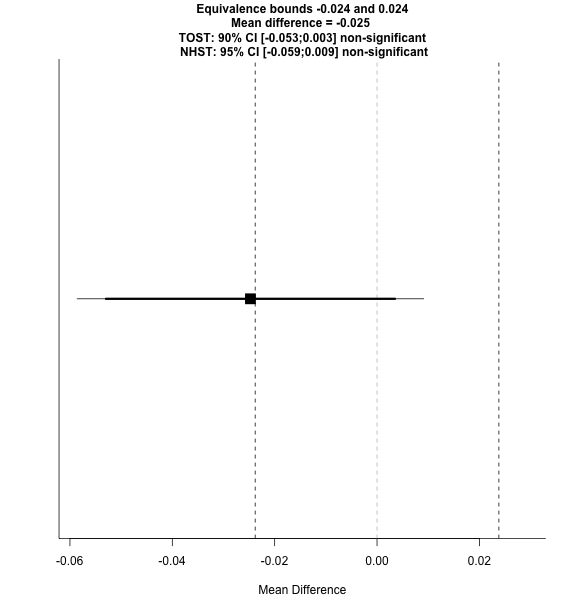
\includegraphics{plots_files/figure-latex/unnamed-chunk-10-1.pdf}

\begin{verbatim}
## TOST results:
## t-value lower bound: -1.60   p-value lower bound: 0.943
## t-value upper bound: -5.13   p-value upper bound: 0.000001
## degrees of freedom : 75.72
## 
## Equivalence bounds (Cohen's d):
## low eqbound: -0.4 
## high eqbound: 0.4
## 
## Equivalence bounds (raw scores):
## low eqbound: -0.0234 
## high eqbound: 0.0234
## 
## TOST confidence interval:
## lower bound 90% CI: -0.067
## upper bound 90% CI:  -0.022
## 
## NHST confidence interval:
## lower bound 95% CI: -0.071
## upper bound 95% CI:  -0.018
## 
## Equivalence Test Result:
## The equivalence test was non-significant, t(75.72) = -1.595, p = 0.943, given equivalence bounds of -0.0234 and 0.0234 (on a raw scale) and an alpha of 0.05.
## Null Hypothesis Test Result:
## The null hypothesis test was significant, t(75.72) = -3.361, p = 0.00122, given an alpha of 0.05.
## Based on the equivalence test and the null-hypothesis test combined, we can conclude that the observed effect is statistically different from zero and statistically not equivalent to zero.
\end{verbatim}

\begin{longtable}[]{@{}lrr@{}}
\toprule
Language & Relative VOT & SD \\
\midrule
\endhead
english & 0.130 & 0.056 \\
french & 0.106 & 0.064 \\
spanish & 0.059 & 0.034 \\
\bottomrule
\end{longtable}

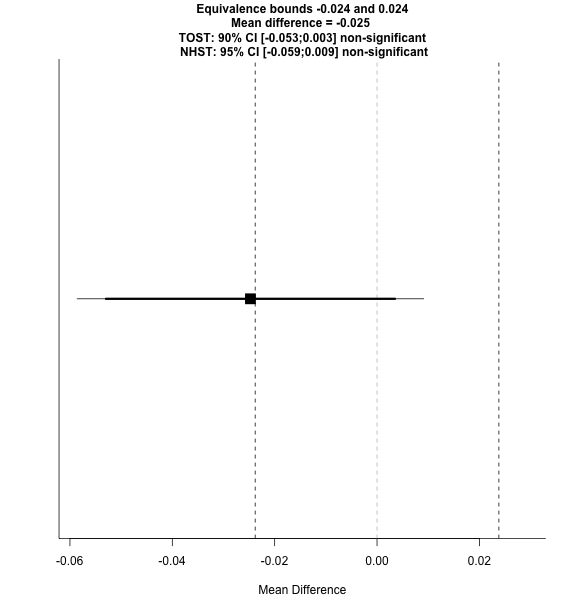
\includegraphics{plots_files/figure-latex/unnamed-chunk-12-1.pdf}

~

relative vot z

Predictors

Estimates

CI

p

(Intercept)

1.14

0.81~--~1.48

\textless0.001

language {[}french{]}

-0.34

-0.67~--~-0.02

0.038

language {[}spanish{]}

-1.19

-1.50~--~-0.87

\textless0.001

text {[}p{]}

-0.96

-1.28~--~-0.63

\textless0.001

text {[}t{]}

-0.68

-1.01~--~-0.36

\textless0.001

Random Effects

σ2

0.35

τ00 word

0.10

τ00 participant

0.17

ICC

0.43

N participant

23

N word

26

Observations

561

Marginal R2 / Conditional R2

0.398 / 0.659

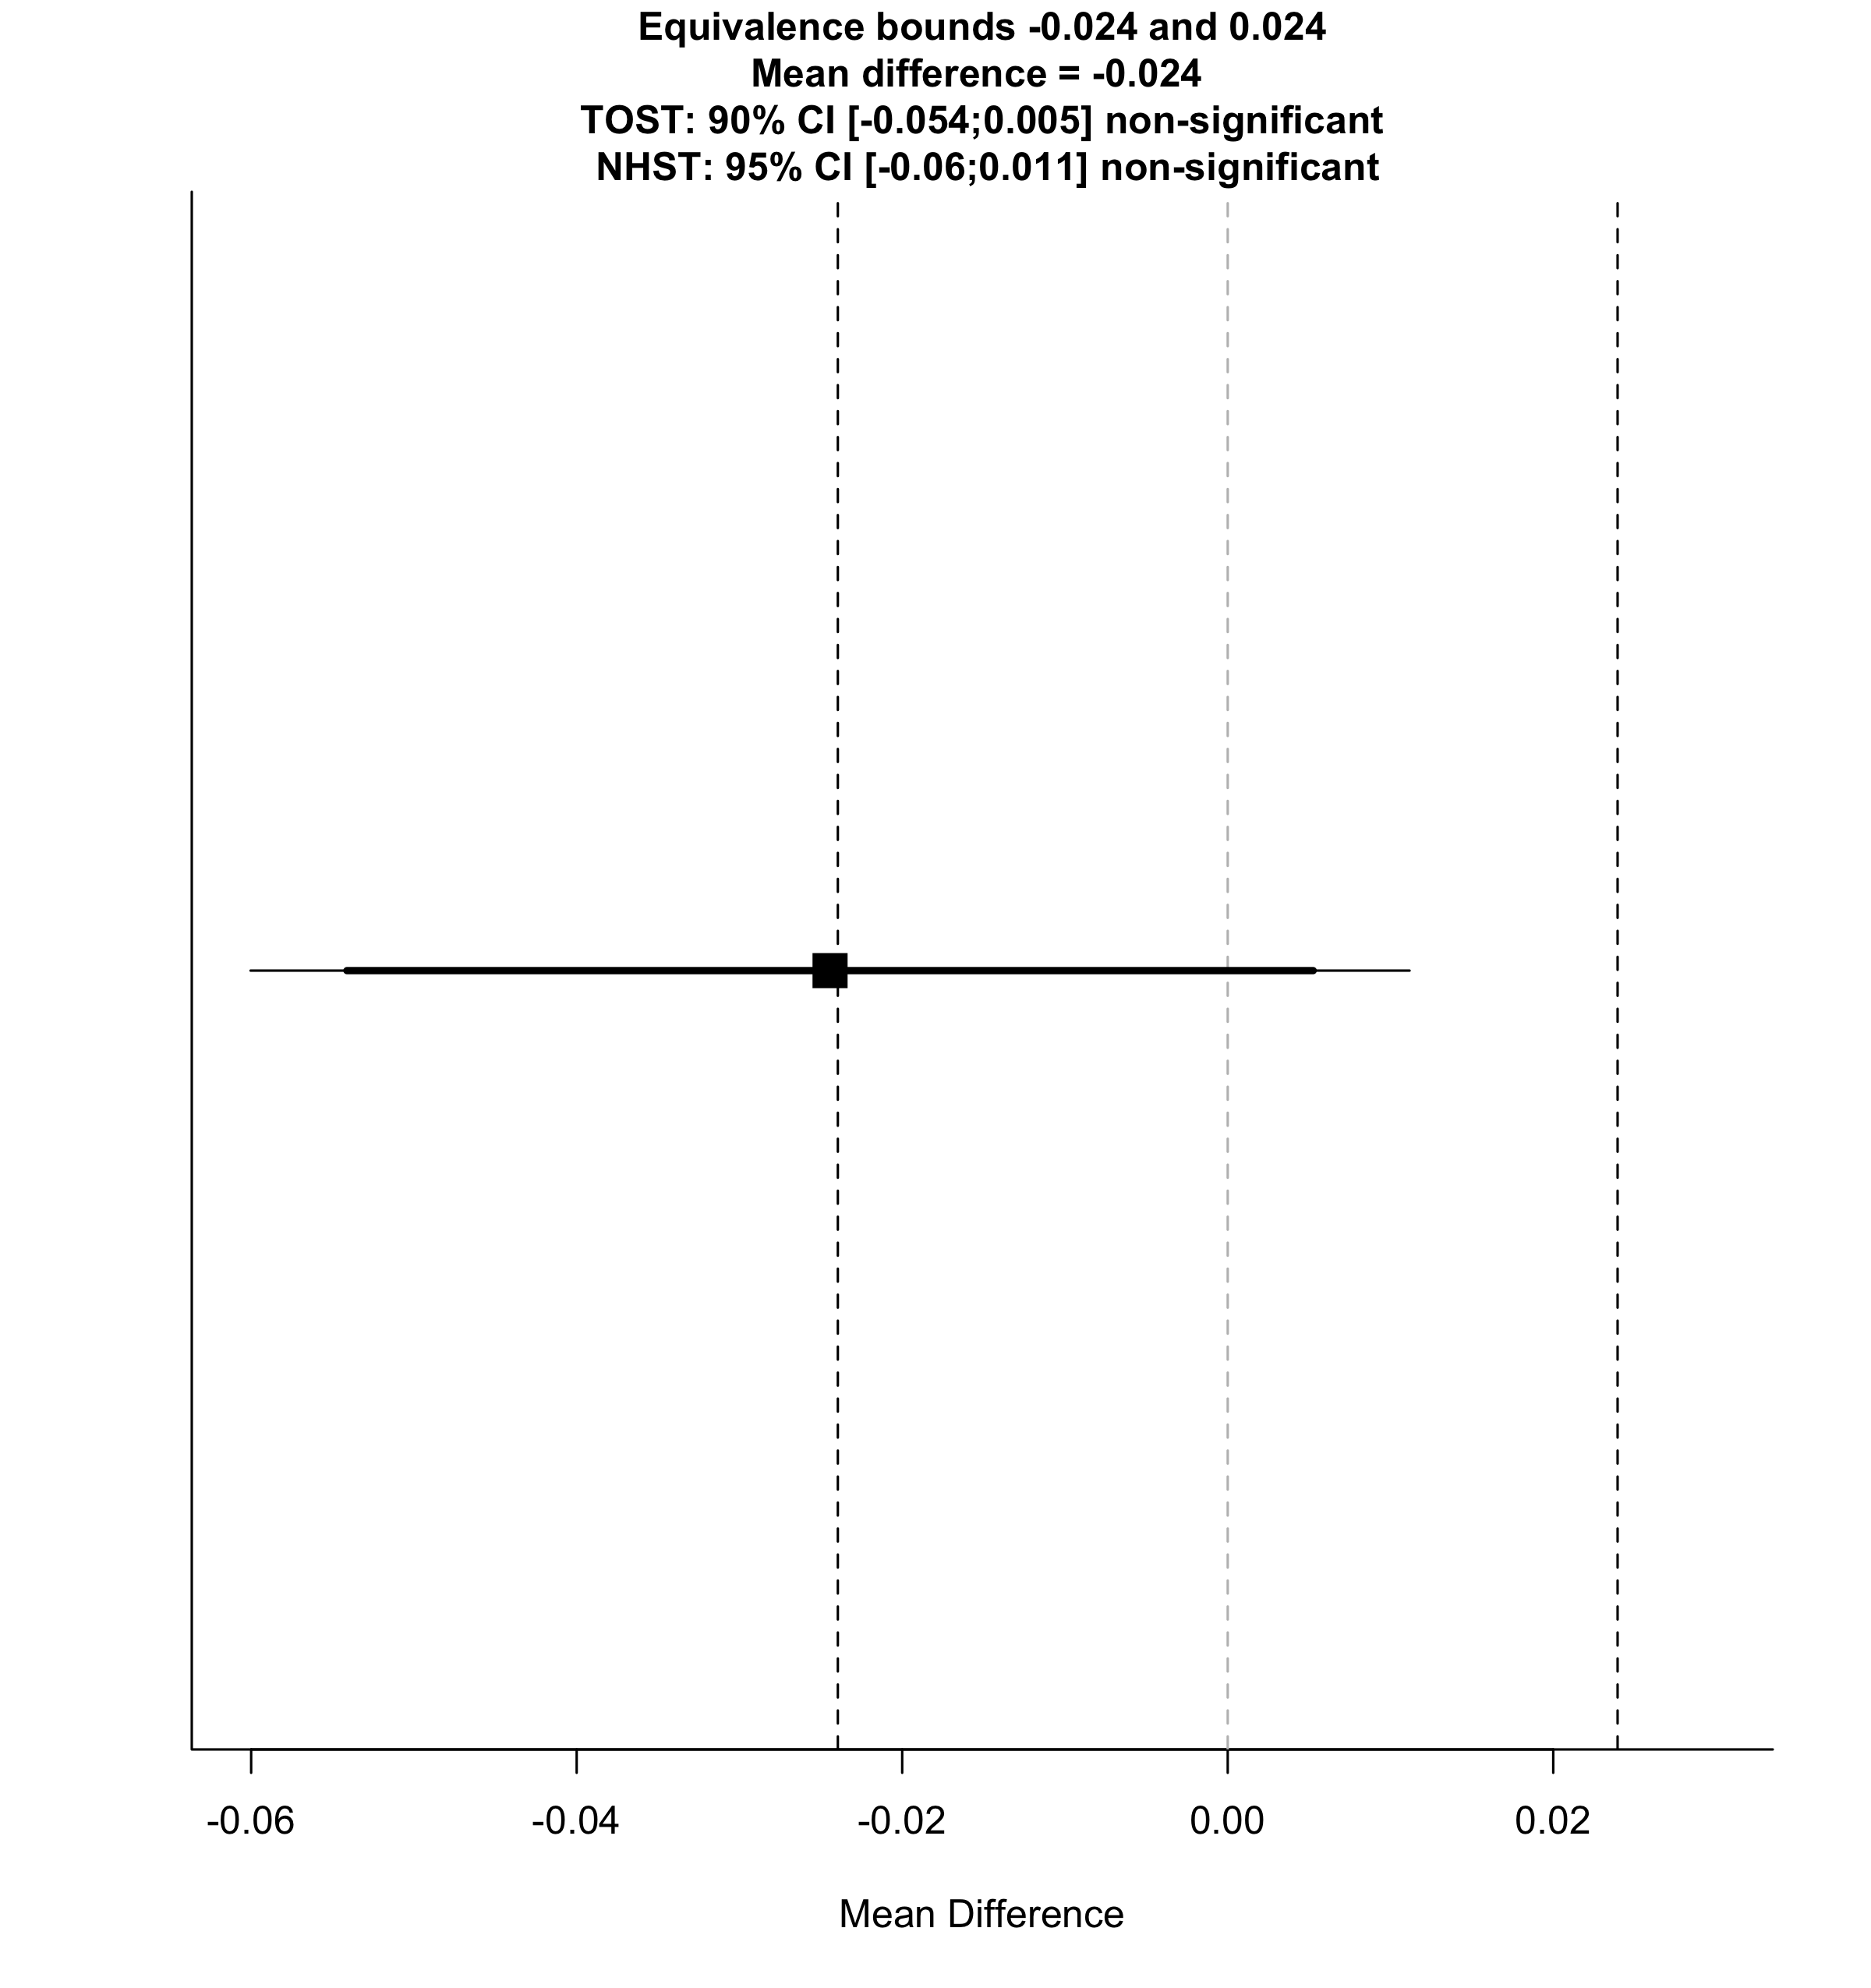
\includegraphics{plots_files/figure-latex/unnamed-chunk-14-1.pdf}

\begin{verbatim}
## TOST results:
## t-value lower bound: 0.0754  p-value lower bound: 0.470
## t-value upper bound: -3.76   p-value upper bound: 0.0005
## degrees of freedom : 22
## 
## Equivalence bounds (Cohen's dz):
## low eqbound: -0.4 
## high eqbound: 0.4
## 
## Equivalence bounds (raw scores):
## low eqbound: -0.0254 
## high eqbound: 0.0254
## 
## TOST confidence interval:
## lower bound 90% CI: -0.047
## upper bound 90% CI:  -0.002
## 
## NHST confidence interval:
## lower bound 95% CI: -0.052
## upper bound 95% CI:  0.003
## 
## Equivalence Test Result:
## The equivalence test was non-significant, t(22) = 0.0754, p = 0.470, given equivalence bounds of -0.0254 and 0.0254 (on a raw scale) and an alpha of 0.05.
## Null Hypothesis Test Result:
## The null hypothesis test was non-significant, t(22) = -1.843, p = 0.0788, given an alpha of 0.05.
## Based on the equivalence test and the null-hypothesis test combined, we can conclude that the observed effect is statistically not different from zero and statistically not equivalent to zero.
\end{verbatim}

\hypertarget{l1-subset-model}{%
\subsubsection{L1 subset model}\label{l1-subset-model}}

\begin{longtable}[]{@{}lrr@{}}
\toprule
Language & Relative VOT & SD \\
\midrule
\endhead
english & 0.140 & 0.058 \\
french & 0.066 & 0.046 \\
spanish & 0.057 & 0.032 \\
\bottomrule
\end{longtable}

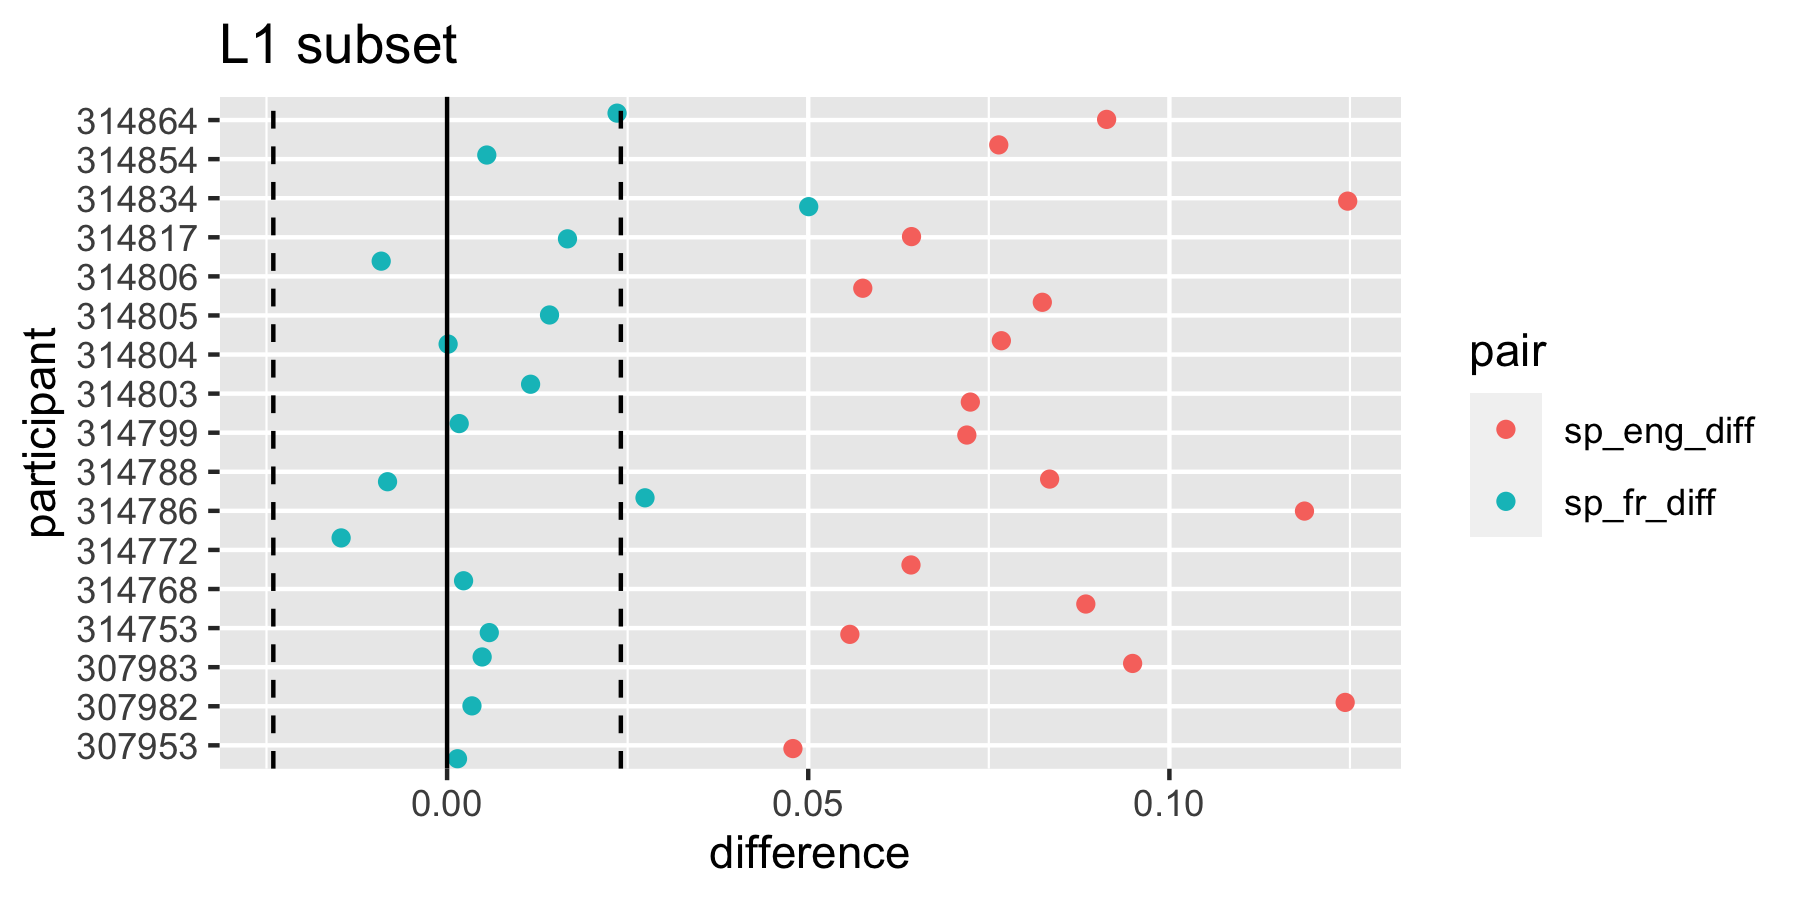
\includegraphics{plots_files/figure-latex/unnamed-chunk-16-1.pdf}

~

relative vot z

Predictors

Estimates

CI

p

(Intercept)

1.31

0.96~--~1.66

\textless0.001

language {[}french{]}

-1.13

-1.43~--~-0.82

\textless0.001

language {[}spanish{]}

-1.39

-1.71~--~-1.07

\textless0.001

text {[}p{]}

-0.94

-1.23~--~-0.65

\textless0.001

text {[}t{]}

-0.70

-0.99~--~-0.41

\textless0.001

Random Effects

σ2

0.28

τ00 word

0.07

τ00 participant

0.23

τ11 participant.languagefrench

0.04

τ11 participant.languagespanish

0.10

ρ01 participant.languagefrench

-1.00

ρ01 participant.languagespanish

-1.00

N participant

16

N word

26

Observations

388

Marginal R2 / Conditional R2

0.657 / NA

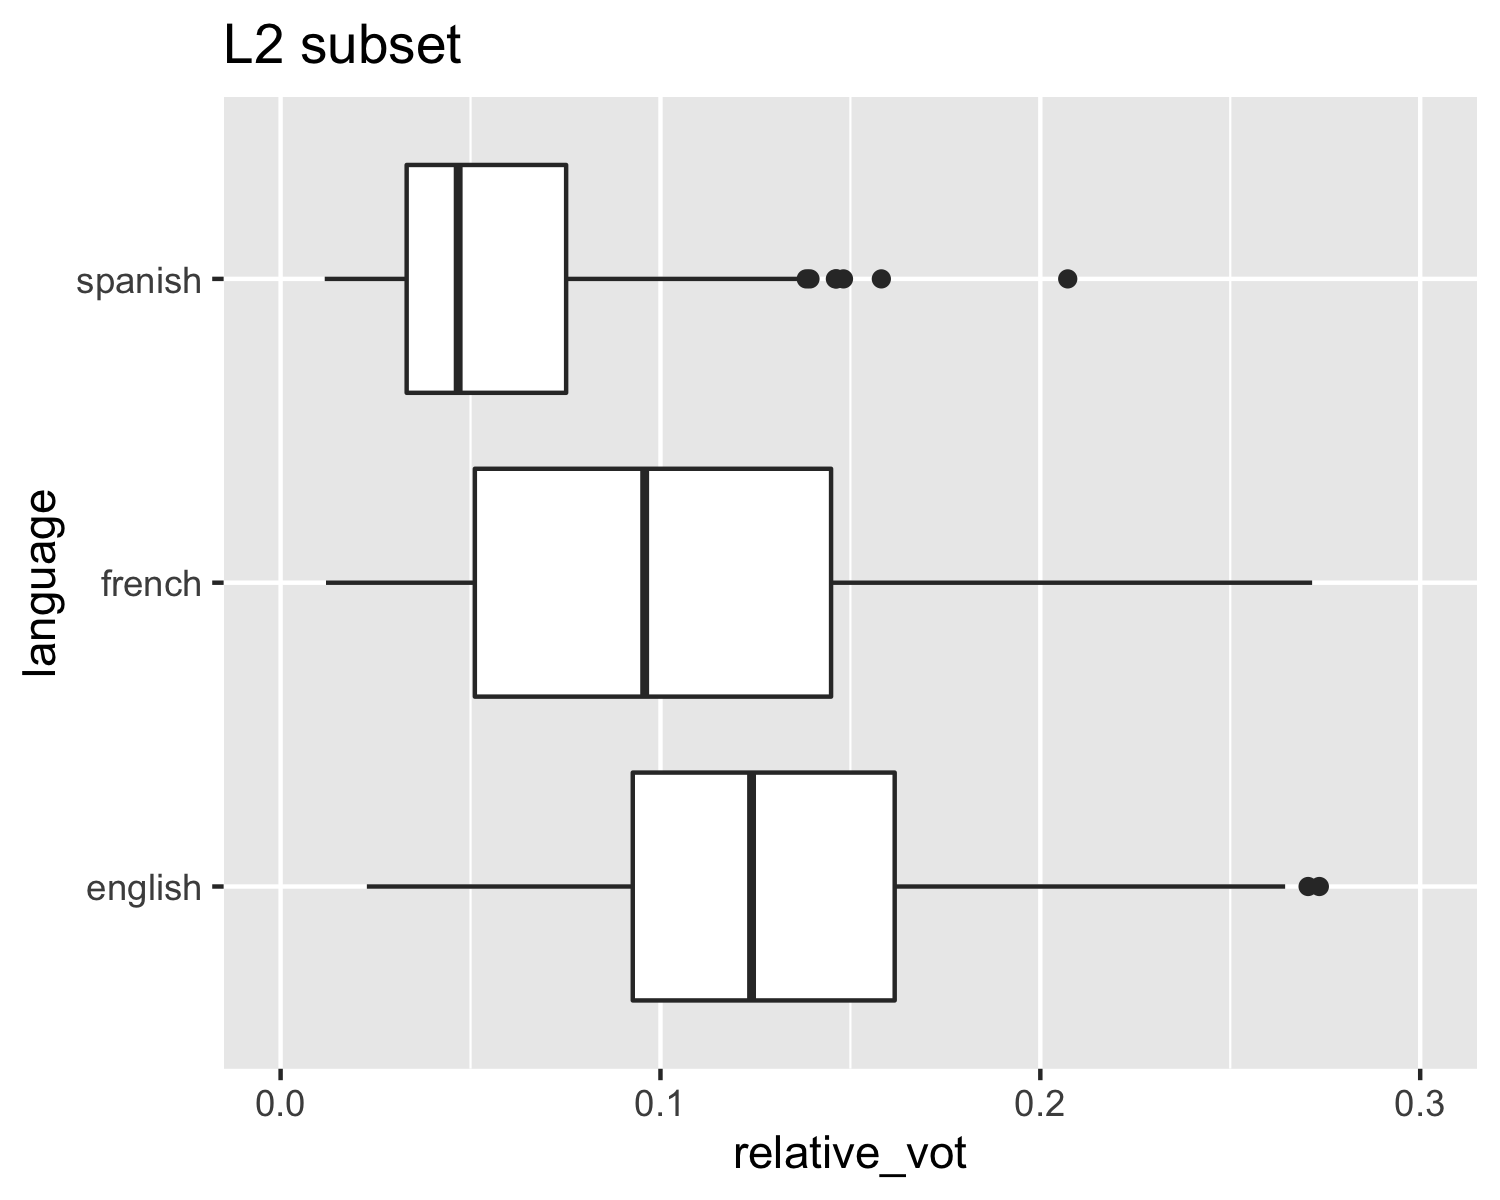
\includegraphics{plots_files/figure-latex/unnamed-chunk-18-1.pdf}

\begin{verbatim}
## TOST results:
## t-value lower bound: 2.43    p-value lower bound: 0.014
## t-value upper bound: -0.773  p-value upper bound: 0.226
## degrees of freedom : 15
## 
## Equivalence bounds (Cohen's dz):
## low eqbound: -0.4 
## high eqbound: 0.4
## 
## Equivalence bounds (raw scores):
## low eqbound: -0.0173 
## high eqbound: 0.0173
## 
## TOST confidence interval:
## lower bound 90% CI: -0.01
## upper bound 90% CI:  0.028
## 
## NHST confidence interval:
## lower bound 95% CI: -0.014
## upper bound 95% CI:  0.032
## 
## Equivalence Test Result:
## The equivalence test was non-significant, t(15) = -0.773, p = 0.226, given equivalence bounds of -0.0173 and 0.0173 (on a raw scale) and an alpha of 0.05.
## Null Hypothesis Test Result:
## The null hypothesis test was non-significant, t(15) = 0.827, p = 0.421, given an alpha of 0.05.
## Based on the equivalence test and the null-hypothesis test combined, we can conclude that the observed effect is statistically not different from zero and statistically not equivalent to zero.
\end{verbatim}

\end{document}
